\capitulo{5}{Aspectos relevantes del desarrollo del proyecto}

\section{Tratamiento de datos}

\subsection{Lectura de datos}

Teniendo en cuenta los objetivos del proyecto ya comentados en apartados anteriores y queriendo lograr la construcción de una aplicación estable para que el usuario final pueda cargar sus datos y administrarlos, nos vimos obligados en primera instancia a buscar una librería en PHP capaz de leer una serie de datos desde un Excel, pues el cliente nos envió los datos en dicho formato, para que en un futuro fuesen administrables y poder ser alojados en nuestra base de datos.

\subsubsection{Phpspreadsheet}

Para realizar esta operación, el alumno conocía una librería llamada \textit{PHPExcel} pero que actualmente a día de hoy está deprecada, por tanto, hubo que investigar y buscar cuál era la solución actualmente. Así se consiguió dar con \textit{Phpoffice/Phpspreadsheet}. Mediante esta librería, que podemos encontrar su documentación en \href{https://phpspreadsheet.readthedocs.io/en/develop/}{phpspreadsheet}~\cite{web:spreadsheet}, se puede realizar lecturas y escrituras sobre un Excel. 

En la figura~\ref{fig:spreadsheet} se puede ver que la librería cubre con creces los requisitos necesarios, además de ofrecer alguna opción extra por si en un futuro o en próximas versiones del proyecto fuesen de interés~\cite{web:spreadsheet}.

\begin{figure}[ht]
	\centering
	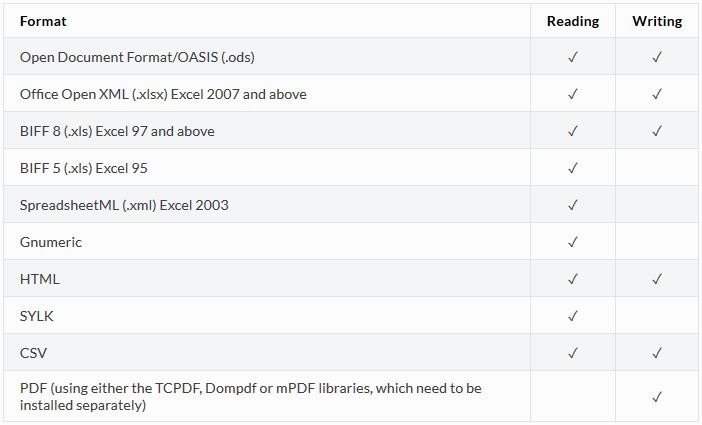
\includegraphics[width=0.9\textwidth]{/aspectosRelevantes/spreadsheet}
	\caption{Formatos de ficheros soportados por Spreadsheet.}
	\label{fig:spreadsheet}
\end{figure}

Para instalar librerías en CakePHP, framework utilizado para el desarrollo del proyecto, hay diversas opciones, pero una de las más sencillas es utilizar \textit{Composer\footnote{Herramienta para la gestión de dependencias en PHP. Le permite declarar y administrar las bibliotecas de las que depende su proyecto.}}.

Para instalar \textit{Spreadsheet} mediante \textit{Composer}, desde el directorio del proyecto ejecutamos:

\begin{lstlisting}[language=bash]
composer require phpoffice/phpspreadsheet
\end{lstlisting}

Una vez la instalada, simplemente con la siguiente linea se puede importar en nuestro proyecto.

\begin{lstlisting}[language=PHP]
use PhpOffice\PhpSpreadsheet\Spreadsheet;
\end{lstlisting}

Como se ve, aunque el trato de los datos y la organización de los mismos si que ha sido un tema delicado, la instalación de las librerías en \textit{CakePHP} es bastante sencilla.

\subsection{Escritura y almacenamiento de los datos}

En cuanto al manejo de los datos, aquí si que ha habido más problemas. Se nos ha juntado la gran cantidad de datos, con que el servidor donde hemos alojado esta primera versión de la aplicación no cuenta con recursos muy elevados.

Ha habido problemas a la hora de subir al servidor archivos muy grandes pues se agotaba la memoria al procesar los datos~\footnote{Rondando las 400K registros.} y se quedaba atascado. 

En nuestro entorno de desarrollo local, el problema del tamaño de los archivos lo solucionamos modificando la propiedad $upload\_max\_file\_size$ en el archivo $php.ini$ pero al no tener acceso a este archivo en el servidor, no podemos modificarlo. 

El problema de la memoria al procesar los datos, no se ha podido solucionar ni con la sentencia $ini\_set('memory\_limit', '-1');$ para indicar que puede utilizar toda la memoria que necesite, ni con la sentencia $set\_time\_limit(0);$ para indicar que tiene el tiempo de ejecución ilimitado. 

Por esta razón es por lo que hemos tenido que fragmentar las cargas y administraciones de ciertos datos aunque lo ideal de cara a la usabilidad del usuario hubiera sido poder hacerlo todo en un mismo paso.

Para almacenar todos estos datos y poder dar al usuario la posibilidad de administrarlos, se ha construido una base de datos relacional. Para gestionarla, se ha utilizado el software \textit{HeidiSQL} que ofrece la posibilidad de conectarse a servidores \textit{MySQL}\footnote{Sistema de gestión de bases de datos relacional}.

\section{Estructura de la aplicación}

La estructura de directorios de nuestro proyecto se puede ver en la figura~\ref{fig:estructuraProyecto}. Destacamos los siguientes directorios:

\begin{itemize}
	\item \textit{config}: En la figura~\ref{fig:estructuraProyectoConfig} vemos los ficheros de configuración de nuestra aplicación. Con una importancia especial podemos destacar: 
	\begin{itemize}
		\item app.php: Archivo donde se establecen los parámetros de configuración para el email, la base de datos, los logs, la sesión, el debug, etc.
		\item constantes.php: Como indica el nombre del archivo, aquí se declaran clases con constantes comunes para poder usarlas desde el resto de la aplicación.
		\item paths.php: Definir variables globales para rutas de directorios concretos.
	\end{itemize}
		
	\item \textit{webroot}: Dentro de la estructura cliente-servidor, en la figura~\ref{fig:estructuraProyectoWebroot} se encuentra lo relacionado con el cliente. Nuestra hoja de estilos, los archivos $*.js$, las imágenes, las fuentes y el favicon.pnp\footnote{Se conoce como favicon al icono que aparece en la pestaña del navegador junto con el nombre de la aplicación.}.
	
	\item \textit{src}: Aquí se almacenarán los archivos de tu aplicación.
\end{itemize}

\begin{figure}[ht]
	\centering
	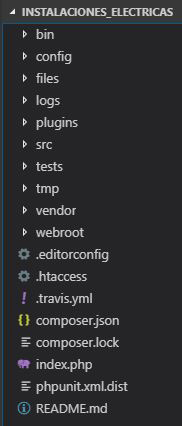
\includegraphics[width=0.3\textwidth]{/aspectosRelevantes/estructuraProyecto}
	\caption{Estructura general de un proyecto desarrollado con CakePHP.}
	\label{fig:estructuraProyecto}
\end{figure}

\begin{figure}[ht]
	\centering
	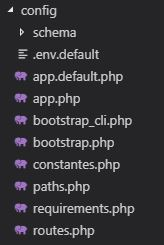
\includegraphics[width=0.3\textwidth]{/aspectosRelevantes/estructuraProyectoConfig}
	\caption{Directorio \textit{config} de nuestro proyecto.}
	\label{fig:estructuraProyectoConfig}
\end{figure}

\begin{figure}[ht]
	\centering
	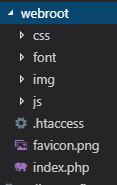
\includegraphics[width=0.2\textwidth]{/aspectosRelevantes/estructuraProyectoWebroot}
	\caption{Directorio \textit{webroot} de nuestro proyecto.}
	\label{fig:estructuraProyectoWebroot}
\end{figure}

No obstante, en la documentación oficial de \textit{CakePHP}~\cite{web:estructuraCarpetasCakePHP} se explican con mayor detalle cada uno de los directorios del proyecto.

\subsection{MVC}

El utilizar \textit{CakePHP} como \textit{framework} ha facilitado mucho la estructura del proyecto pues trabaja con el patrón MVC. De esta manera, como podemos ver en la figura \ref{fig:estructuraProyectoSrc}, tenemos bien separadas las tres partes fundamentales de la aplicación. 

\begin{figure}[ht]
	\centering
	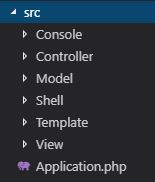
\includegraphics[width=0.2\textwidth]{/aspectosRelevantes/estructuraProyectoSrc}
	\caption{Directorio \textit{src} de nuestro proyecto.}
	\label{fig:estructuraProyectoSrc}
\end{figure}

Por un lado tenemos la conexión con nuestra base de datos en lo que serían los \textit{modelos}\footnote{Directorio \textit{Models}.}. Allí están la mayoría de consultas y operaciones contra la base de datos. 

Por otro lado tenemos la parte de los \textit{controladores}\footnote{Directorio \textit{Controller}.}. que hacen de intermediarios entre la base de datos y la vista. Aquí albergamos la parte lógica de nuestra aplicación.

Por último las \textit{vistas}\footnote{Directorio \textit{Templates}.}. Esto es lo que ve el usuario. Como ya hemos comentado, para facilitarnos el trabajo y aprovechar herramientas muy útiles ya creadas y puestas en el mercado, hemos utilizado \textit{Foundation 6.4.2}

Su implementación dentro del proyecto es muy sencilla, simplemente tenemos que colocar la siguiente linea en el \textit{layout\footnote{Vista definida como plantilla común al resto de vistas.}}:

\begin{lstlisting}[language=php]
echo $this->Html->css('lib/foundation-6.4.2/css/foundation.css');
\end{lstlisting}